\chapter{Theoretical Results}\label{ch:theoretical_results}
Based on the definitions in the previous chapter, we will prove a few theorems necessary for the implementation of the solvers. First of all, we will show that it suffices to check the coverage of the shadow witness set instead of all AVPs, which greatly reduces the size of the formulations for the CAGP.

\begin{theorem}[Couto et al.~\cite{couto2011exact}]\label{thm:shadow_coverage}
When given a polygon $P$ and a guard set $G$, a subset $G_{sub}$ of $G$ fully covers $P$ if and only if it covers all witnesses in the shadow witness set $W$ of $G$. 
\end{theorem}
\begin{proof}
The necessity condition follows trivially from $W\subset P$. As for the sufficiency condition, consider the largest area $R$ that is not covered by $G_{sub}$. Because of the atomicity of AVPs, $R$ must consist of one or more AVPs. Now consider the AVP $f$ with minimal guard subset $G_{f}$ in $R$. We show that $f$ must be a shadow AVP, a contradiction. If $f = R$, then $f$ must trivially be a shadow AVP. Otherwise, consider the neighbors of $f$. For all neighbors in $R$, $G_{f}$ can not contain their guard subset as $G_{f}$ is minimal in $R$. As for the neighbors not in $R$, if there exists a neighbor of which the guard subset is contained in $G_{f}$, then $f$ must be covered by one of the guards in that subset and can not be part of $R$. Otherwise, $G_{f}$ does not contain any of its neighbors' guard subsets and thus is a shadow AVP.
\end{proof}

Next, we will show that instead of creating the 2-link-visibility graph $G_{vis}$ from checking for an intersection between all combinations of guard visibility polygons, we can use the guard subsets of the light AVPs. This greatly reduces the graph creation time as many polygon operations can be expensive.

\begin{theorem}\label{thm:light_covers}
When given a polygon $P$ and a guard set $G$, the guard subsets of a light polygon form a clique in the 2-link-visibility graph $G_{vis}$ of $G$, and the cliques of all light polygons cover all edges of $G_{vis}$.
\end{theorem}
\begin{proof}
The guard subset of a light polygon is formed by all the guards whose visibility polygons intersect in it, thus trivially forming a clique in $G_{vis}$. Assuming that for $g,g'\in G$ there exists an edge $(g, g')$ in $G_{vis}$ that is not covered by those cliques, then there exists an AVP $f$ that is not light and contains $g$ and $g'$ in its guard subset $G_{sub}$. As $f$ is not light there exists a neighboring AVP $f'$ whose guard subset contains $G_{sub}$. One can continue this argument with $f'$, but as the number of AVPs is finite, we will eventually reach an AVP $f^{*}$ of which the guard subset is not contained in its neighbors. Thus, $f^{*}$ is a light AVP and contains $g$ and $g'$, a contradiction.
\end{proof}

\begin{figure}[htbp]
\centering
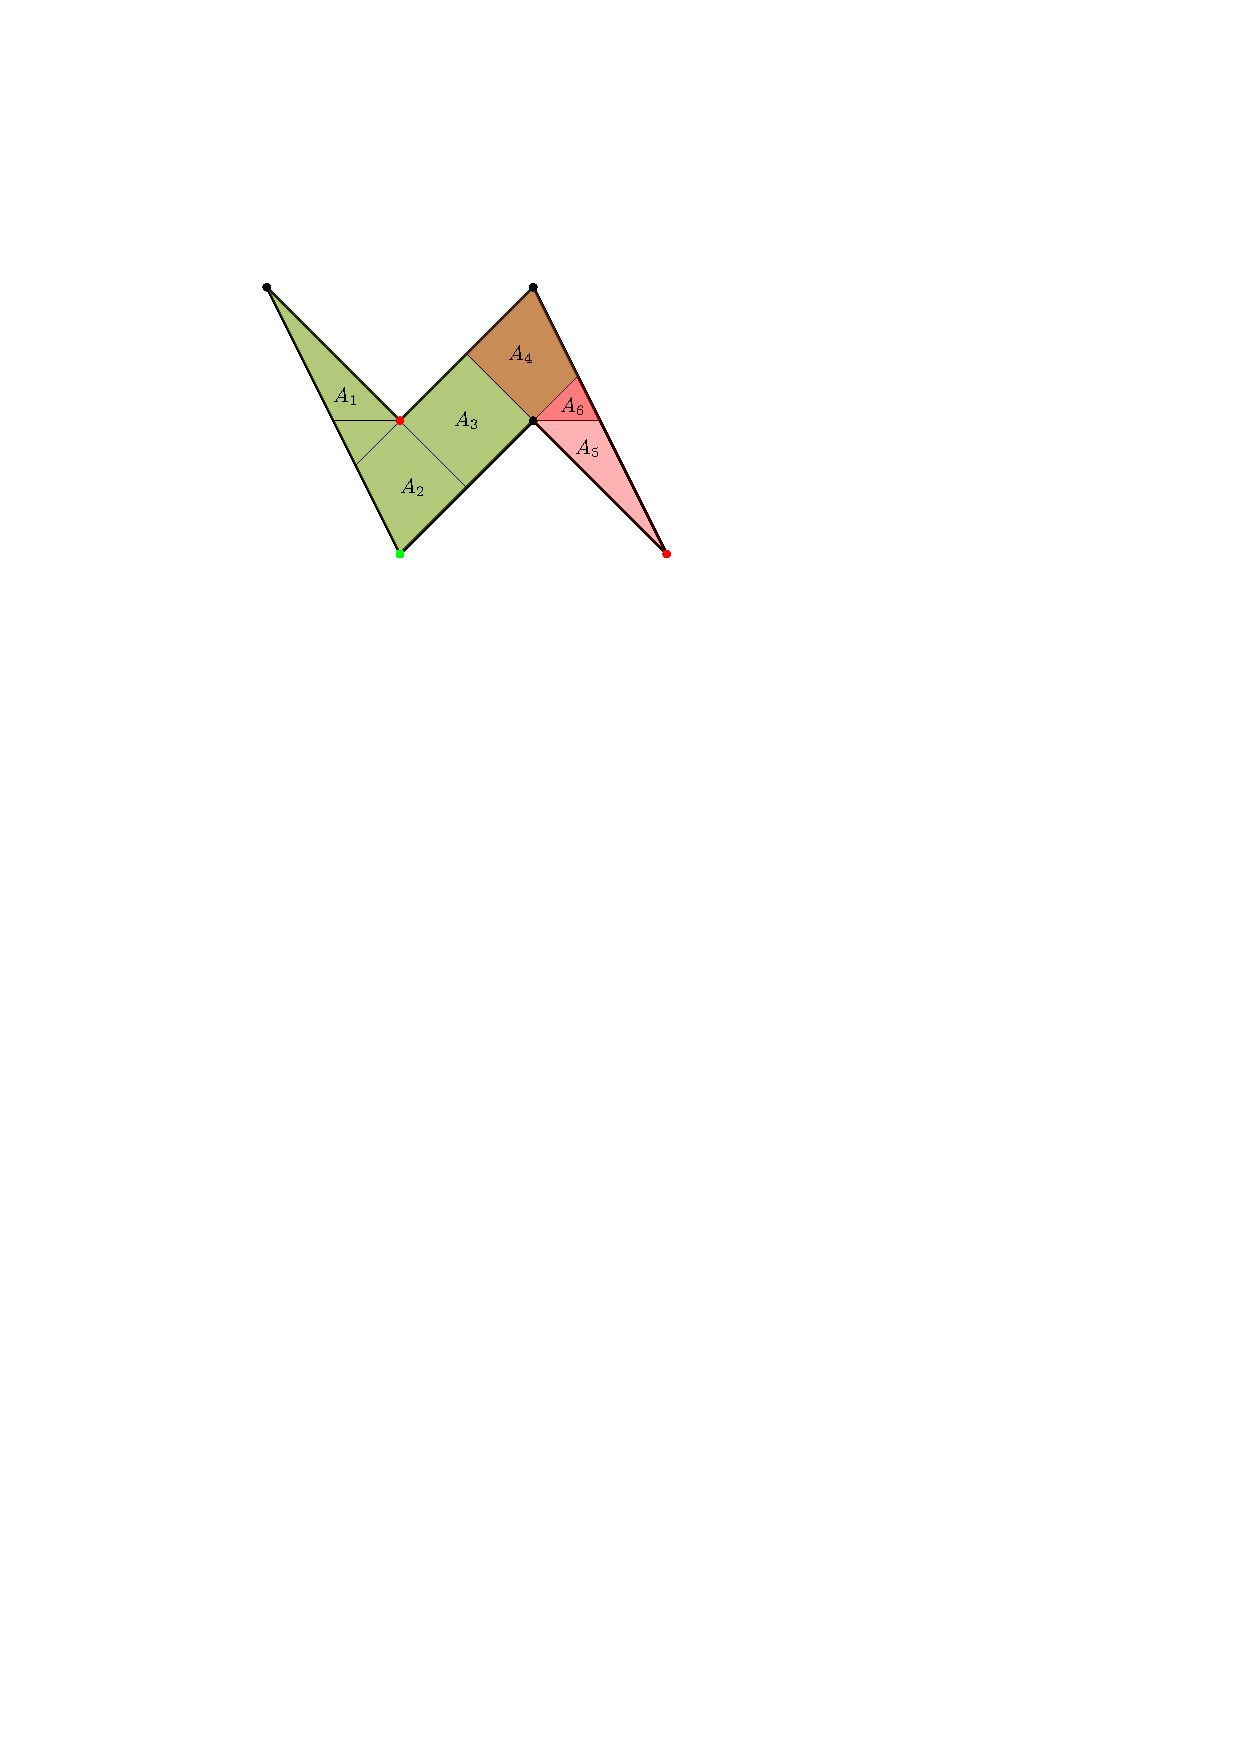
\includegraphics[scale=1.3]{Thesis/figures/conflict-free_witnesses_updated.pdf}
\caption{Illustration for the proof of \cref{thm:conflict-free_witnesses}.}
\label{fig:conflict-free_witnesses}
\end{figure}

Lastly, we will prove that, unlike the CAGP, we cannot restrict ourselves to either shadow or light witness set to check the conflict-freeness for the CFCAGP.

\begin{theorem}\label{thm:conflict-free_witnesses}
For a polygon $P$ and a guard set $G$, neither conflict-freeness of all shadow witnesses nor all light witnesses guarantees conflict-freeness within all AVPs even if restricted to an optimal number of colors.
\end{theorem}
\begin{proof}
To prove this theorem, we present a simple example in \cref{fig:conflict-free_witnesses}. By placing a witness in the center of $A_{1}$ and $A_{5}$, we get two independent witnesses, meaning we need at least two guards to cover the entire polygon. As for any guard set with two or more vertices, there exists at least one pair of guards whose visibilities intersect, we require at least two colors. $A_{1}$, $A_{3}$ and $A_{5}$ are shadow AVPs and $A_{2}$ and $A_{4}$ are light AVPs. Each of them is covered by at least one guard of unique color. On the other hand, $A_{6}$ is neither shadow nor light and is only covered by two guards of the same color, thus, it is not conflict-free.
\end{proof}

\chapter{Chromatic Art Gallery Problem Formulations}

In the following sections, we introduce a MIP, a SAT, and a CP-SAT formulation of the Chromatic Art Gallery Problem. The MIP formulation is the one proposed by Zambon et al.~\cite{zambon2014exact}, which gets modified and turned into a SAT formula for the SAT and the CP-SAT formulation.

\section{MIP Formulation}

\begin{align}
\label{eq_MIP:f.0} \mbox{minimize}~& \;\sum_{k\in \{1,\ldots,K\}} c_{k}& \\
\label{eq_MIP:f.1} \mbox{s.t. } &\sum_{g \in H}x_{gk} \leq c_{k} & \forall H \in \mathcal{H}, \forall k\in \{1,\ldots,K\}\\
\label{eq_MIP:f.2}&\sum_{g\in N(w), k\in \{1,\ldots,K\}}x_{gk}\geq 1 & \forall w\in W\\
\label{eq_MIP:f.3}&\sum_{k\in \{1,\ldots,K\}}x_{gk}\leq1 & \forall g\in G\\
\label{eq_MIP:f.4}&c_{k} - c_{k+1} \geq 0 & \forall k\in \{1,\ldots,K-1\}\\
\label{eq_MIP:f.5}&\sum_{g\in G}x_{gk} - \sum_{g\in G}x_{g(k+1)} \geq 0 & \forall k\in \{1,\ldots,K-1\}\\
\label{eq_MIP:f.6}& x_{gk} \in \{0,1\} & \forall g\in G, \forall k\in \{1,\ldots,K\}\\
\label{eq_MIP:f.7}& c_{k}\in \{0,1\} & \forall k\in \{1,\ldots,K\}
\end{align}

The MIP formulation of the problem introduces binary variables for every guard color combination \cref{eq_MIP:f.6} and every color \cref{eq_MIP:f.7}. The guard color variables are true whenever the guard is used and is assigned the associated color in the solution. The color variables are true whenever a guard uses that color in a solution. The objective function \cref{eq_MIP:f.0} minimizes the number of colors used in the solution. The constraints in \cref{eq_MIP:f.1} are called clique edge cover constraints. They ensure that for every clique in a clique edge cover of the 2-link-visibilty-graph $G_{vis}$ and every color only one of the guards in that clique can be assigned that color. At the same time, they make sure that if a guard in that clique uses the color, the corresponding color variable must also be true. How to find a clique edge cover for $G_{vis}$, will be discussed in the Implementation Details chapter. The constraints in \cref{eq_MIP:f.2} are called witness covering constraints. They ensure that for every witness in the witness covering graph $G_{cov}$ at least one guard in its neighborhood is used in the solution, thus the witness gets covered. We call the constraints in \cref{eq_MIP:f.3} guard coloring constraints. They ensure that each guard is assigned at most one color. Technically, these constraints are not necessary to find an optimal solution, as one can simply process the solution by deciding on one color for every guard that got assigned multiple. The reason for still including these constraints is that they reduce the space of possible optimal and near-optimal solutions, which can help the solver arrive at an optimal solution faster. In the same mindset, we add the constraints \cref{eq_MIP:f.4} and \cref{eq_MIP:f.5}, which are symmetry breaker constraints. \cref{eq_MIP:f.4} ensure that when $k$ colors are used, those colors are the first k colors in $\{1,\ldots,K\}$. As for \cref{eq_MIP:f.4}, they induce a partial order of the colors over the size of guards using that color. This reduces the possible permutations of the colors assigned to each guard in an optimal solution.

\section{SAT Formulation}

\begin{align}
\label{eq_SAT:f.0}&\lnot x_{uk} \lor \lnot x_{vk} & \forall (u,v)\in E_{G_{vis}}, \forall k\in \{1,\ldots,K\}\\
\label{eq_SAT:f.1}&\bigvee_{g\in N(w), k\in \{1,\ldots,K\}}x_{gk} & \forall w\in W\\
\label{eq_SAT:f.2}&\bigwedge_{1 \leq i < j \leq K} (\lnot x_{gi} \lor \lnot x_{gj}) & \forall g\in G\\
\label{eq_SAT:f.3}& x_{gk} \in \{0,1\} & \forall g\in G, \forall k\in \{1,\ldots,K\}
\end{align}

The SAT formulation of the problem differs from the MIP formulation in the way that we are not trying to minimize the number of colors used. Instead, we test whether there exists a feasible solution given a fixed number of colors K. By doing so, we can solve the SAT formula for different numbers of colors, increasing the number whenever we encounter infeasibility and decreasing it on a feasible solution, until we find the smallest number of colors for which there exists a feasible solution. The exact procedure for choosing the number of colors will be discussed in the Implementation Details chapter. Because we have a fixed number of colors, we do not require color variables like \cref{eq_MIP:f.7} anymore and restrict ourselves to the guard color variables in \cref{eq_SAT:f.3}. We also omit the symmetry breaker constraints \cref{eq_MIP:f.4} and \cref{eq_MIP:f.5}, as \cref{eq_MIP:f.4} uses color variables and we found no straightforward way to model them efficiently using SAT clauses. Now for the clauses in our SAT formulation, we ensure that no two guards that share an edge in the 2-link-visibility graph $G_{vis}$ share the same color using \cref{eq_SAT:f.0}. These clauses replace the clique edge cover constraints in \cref{eq_MIP:f.1}. The reason for simply using the edges of $G_{vis}$ and not cliques is that SAT solvers are very efficient at solving large numbers of small clauses, i.e., with only two variables. For the witness covering constraints \cref{eq_MIP:f.2}, we use the clauses in \cref{eq_MIP:f.1}, which have an equivalent meaning. Lastly, we use the clauses in \cref{eq_MIP:f.2} to replace the guard coloring constraints in \cref{eq_MIP:f.3}. Again, these constraints can be omitted by processing the solution at the end and we will compare the performance with and without them in the Experiments chapter below.

\section{CP-SAT Formulation}

As CP-SAT solvers allow for both MIP and SAT constraints, we use both the MIP and the SAT formulation and compare them against each other in the Experiments chapter.

\chapter{Conflict-free Chromatic Art Gallery Problem Formulations}

In the following sections, we introduce a MIP and a SAT formulation of the Conflict-free Chromatic Art Gallery Problem.

\section{MIP Formulation}

\begin{align}
\label{eq_MIP_cf:f.0} \mbox{minimize}~& \;\sum_{k\in \{1,\ldots,K\}} c_{k}& \\
\label{eq_MIP_cf:f.1} \mbox{s.t. } &\sum_{g \in G}x_{gk} \geq c_{k} & \forall k\in \{1,\ldots,K\}\\
\label{eq_MIP_cf:f.2}&\sum_{g\in G}x_{gk} \leq |G|\cdot  c_{k} & \forall k\in \{1,\ldots,K\}\\
\label{eq_MIP_cf:f.3}&\sum_{g\in N(w)}x_{gk} \geq u_{wk} & \forall w\in W, \forall k\in \{1,\ldots,K\}\\
\label{eq_MIP_cf:f.4}&\sum_{g\in N(w)}x_{gk} \leq 1 + |N(w)|\cdot  (1-u_{wk}) & \forall w\in W, \forall k\in \{1,\ldots,K\}\\
\label{eq_MIP_cf:f.5}&\sum_{k\in \{1,\ldots,K\}}u_{wk} \geq 1 & \forall w\in W\\
\label{eq_MIP_cf:f.6}&\sum_{k\in \{1,\ldots,K\}}x_{gk} \leq 1 & \forall g\in G\\
\label{eq_MIP_cf:f.7}&c_{k} - c_{k+1} \geq 0 & \forall k\in \{1,\ldots,K-1\}\\
\label{eq_MIP_cf:f.8}&\sum_{g\in G}x_{gk} - \sum_{g\in G}x_{g(k+1)} \geq 0 & \forall k\in \{1,\ldots,K-1\}\\
\label{eq_MIP_cf:f.10}& u_{wk} \in \{0,1\} & \forall w\in W, \forall k\in \{1,\ldots,K\}\\
\label{eq_MIP_cf:f.11}& x_{gk} \in \{0,1\} & \forall g\in G, \forall k\in \{1,\ldots,K\}\\
\label{eq_MIP_cf:f.12}& c_{k}\in \{0,1\} & \forall k\in \{1,\ldots,K\}
\end{align}

The MIP formulation for the CFCAGP is similar to the one of the CAGP. We are still trying to minimize the number of colors \cref{eq_MIP_cf:f.0} and keep the same variables \cref{eq_MIP_cf:f.11} for colors and \cref{eq_MIP_cf:f.12} for guard color combinations. Additionally, we add auxiliary variables \cref{eq_MIP_cf:f.10}, called unique color witness variables, for all witness color combinations. They are true whenever there exists exactly one guard with that color in the neighborhood of that witness. To ensure that the color variables are true if and only if a guard variable of that color is true, we add the constraints in \cref{eq_MIP_cf:f.1} and \cref{eq_MIP_cf:f.2}. The constraints \cref{eq_MIP_cf:f.3} and \cref{eq_MIP_cf:f.4} ensure that if a unique color witness variable is true, exactly one guard in the neighborhood of that witness has that color. Otherwise, there can be arbitrarily many guards of that color in the neighborhood. Lastly, we keep the guard coloring constraints \cref{eq_MIP_cf:f.6} and symmetry breaker constraints \cref{eq_MIP_cf:f.7} and \cref{eq_MIP_cf:f.8} of the CAGP MIP Formulation.

\section{SAT Formulation}

\begin{align}
\label{eq_SAT_cf:f.0}&\lnot u_{wk} \lor \bigvee_{g \in N(w)}x_{gk} & \forall w \in W, \forall k\in \{1,\ldots,K\}\\
\label{eq_SAT_cf:f.1}&\bigwedge_{(i,j)\in {G\choose 2}} (\lnot u_{wk} \lor \lnot x_{ik} \lor \lnot x_{jk}) & \forall w \in W, \forall k\in \{1,\ldots,K\}\\
\label{eq_SAT_cf:f.2}&\bigvee_{k\in \{1,\ldots,K\}}u_{wk} & \forall w\in W\\
\label{eq_SAT_cf:f.3}&\bigwedge_{1 \leq i < j \leq K} (\lnot x_{gi} \lor \lnot x_{gj}) & \forall g\in G\\
\label{eq_SAT_cf:f.4}& u_{wk} \in \{0,1\} & \forall w\in W, \forall k\in \{1,\ldots,K\}\\
\label{eq_SAT_cf:f.5}& x_{gk} \in \{0,1\} & \forall g\in G, \forall k\in \{1,\ldots,K\}
\end{align}

For the SAT formulation of the CFCAGP, we test the feasibility of the SAT formula for a fixed K in the same fashion as for the CAGP, until we find a feasible solution with a minimal number of colors. We again omit the color variables and keep the unique color witness variables \cref{eq_SAT_cf:f.4} and guard color variables \cref{eq_SAT_cf:f.5}. The clauses \cref{eq_SAT_cf:f.0} are equivalent to the constraints in \cref{eq_MIP_cf:f.3}. For all witness color combinations, if the unique color witness variable of that color and that witness is true, at least one guard of the color in the neighborhood of that witness has to be true. The clauses \cref{eq_SAT_cf:f.1} are equivalent to the constraints in \cref{eq_MIP_cf:f.4}. For all witness color combinations, if the unique color witness variable of that color and that witness is true, no two guards in the neighborhood of that witness can have that color. As for \cref{eq_SAT_cf:f.2}, these clauses represent the constraints in \cref{eq_MIP_cf:f.5}. Lastly, the witness coloring constraints \cref{eq_SAT_cf:f.3} are modeled using the same clauses as in the CAGP SAT Formulation.

% \section{CP-SAT Formulation}
% Similar to the Chromatic Art Gallery Problem, we use both the MIP and the SAT formulation for CP-SAT and compare them against each other in the Experiments chapter.

\chapter{Implementation Details}\label{ch:implementation_details}

\section{Instance Processing}
The instances are given as lists of points, which represent the outer boundaries of the polygons and possible holes. First, we create a CGAL Polygon\_with\_holes\_2 using the instance input. Then, using the vertices of the polygon and its holes as the guard set $G$, we calculate the visibility regions as polygons for each guard using CGAL's ``Triangular\_expansion\_visibility\_2.h'' and save each guard together with its visibility polygon in a list. Afterward, we recursively overlay the visibility polygons using CGAL's ``Arr\_overlay\_2.h'' to obtain the AVP arrangement (\cref{alg:AVP_generation}). To be able to form the partial order over the AVPs, we overload the overlay function to save for every face a set of guards from which it was created. 

\begin{algorithm}
\caption{AVP Generation}\label{alg:AVP_generation}
\fontsize{10}{12}\selectfont
\begin{algorithmic} 
\Procedure{Generate AVP Recursive}{guards}
\If{len(guards) = $1$}
    \State guard\_id $\gets$ id of the remaining guard
    \State guard\_vis\_poly $\gets$ visibility polygon of the remaining guard
    \State \Return Arrangement(guard\_id, guard\_vis\_poly)
\Else
    \State half $\gets$ len(guards)/$2$
    \State first\_half $\gets$ first half of guards
    \State second\_half $\gets$ second half of guards
    \State AVP\_$1$ $\gets$ Generate AVP Recursive(first\_half)
    \State AVP\_$2$ $\gets$ Generate AVP Recursive(second\_half)
    \State \Return AVP\_$1$.overlay(AVP\_$2$)
\EndIf
\EndProcedure
\end{algorithmic}
\end{algorithm}

For the CAGP, we calculate the shadow witness set. As geometric operations are expensive, instead of saving the shadow witness set as a set of points, we store each witness as an integer together with the set of guards that covers the witness as well as each guard together with the set of witnesses that the guard covers. Additionally, we store a list of the set of guards for each light AVP (\cref{alg:AVP_processing}). For the CFCAGP, we calculate the witness set as well. But because of \cref{thm:conflict-free_witnesses} just using shadow or light witnesses is not sufficient, thus we use a witness for every AVP instead (\cref{alg:AVP_processing_cf}). Afterward, we can use the light guard sets to create the visibility graph $G_{vis}$ by adding edges between guards within each set (\cref{thm:light_covers}). As for the covering graph $G_{cov}$, there is no need to create the overhead of an additional graph. Instead, we can check a witness's corresponding guard set whenever we need that witness's neighborhood in $G_{vis}$. Lastly, we can sort the witnesses by the size of their guard sets and use the $|G|$ smallest witnesses as our initial witnesses.

% \begin{algorithm}
% \caption{Calculate witness sets and light guard sets}\label{alg:AVP_processing}
% \begin{algorithmic}[1]
% \Procedure{AVP Processing}{faces of the AVP arrangement}
% \State Initialize empty maps: shadow\_witness\_to\_guards, guard\_to\_shadow\_witnesses, all\_witness\_to\_guards, guard\_to\_all\_witnesses
% \State Initialize empty list: light\_guard\_sets
% \State shadow\_index $\gets 0$
% \State all\_index $\gets 0$
% \For{face in faces}
%     \State g\_data $\gets$ guard set of the face
%     \If{g\_data is empty}
%         \State Continue
%     \EndIf
%     \State is\_shadow $\gets$ true
%     \State is\_light $\gets$ true
%     \For{half\_edge in face}
%         \State twin\_g\_data $\gets$ guard set of the twin face of the half\_edge
%         \If{twin\_g\_data is empty}
%             \State Continue
%         \EndIf
%         \If{g\_data $\subset$ twin\_g\_data}
%             \State is\_shadow $\gets$ false
%         \EndIf
%         \If{twin\_g\_data $\subset$ g\_data}
%             \State is\_light $\gets$ false
%         \EndIf
%     \EndFor
%     \State all\_witness\_to\_guards[all\_index] $\gets$ g\_data
%     \For{g in g\_data}
%         \State guard\_to\_all\_witnesses[g] $\gets$ guard\_to\_all\_witnesses[g] $\cup$ all\_index
%     \EndFor
%     \State all\_index $\gets$ all\_index + $1$
%     \If{is\_shadow}
%         \State shadow\_witness\_to\_guards[index] $\gets$ g\_data
%         \For{g in g\_data}
%             \State guard\_to\_shadow\_witnesses[g] $\gets$ guard\_to\_shadow\_witnesses[g] $\cup$ index
%         \EndFor
%         \State shadow\_index $\gets$ shadow\_index + $1$
%     \EndIf
%     \If{is\_light}
%         \State light\_guard\_sets.append(g\_data)
%     \EndIf
% \EndFor
% \State \Return shadow\_witness\_to\_guards, guard\_to\_shadow\_witnesses, light\_guard\_sets, all\_witness\_to\_guards, guard\_to\_all\_witnesses
% \EndProcedure
% \end{algorithmic}
% \end{algorithm}

\begin{algorithm}
\caption{AVP Processing (CAGP)}\label{alg:AVP_processing}
\fontsize{10}{12}\selectfont
\begin{algorithmic}[1]
\Procedure{Get shadow witnesses and light guard sets}{AVP arrangement}
\State Initialize empty maps: shadow\_witness\_to\_guards, guard\_to\_shadow\_witnesses
\State Initialize empty list: light\_guard\_sets
\State shadow\_index $\gets 0$
\For{face in faces of the AVP arrangement}
    \State g\_data $\gets$ guard set of the face
    \If{g\_data is empty}
        \State Continue
    \EndIf
    \State is\_shadow $\gets$ true
    \State is\_light $\gets$ true
    \For{half\_edge in face}
        \State twin\_g\_data $\gets$ guard set of the twin face of the half\_edge
        \If{twin\_g\_data is empty}
            \State Continue
        \EndIf
        \If{g\_data $\subset$ twin\_g\_data}
            \State is\_shadow $\gets$ false
        \EndIf
        \If{twin\_g\_data $\subset$ g\_data}
            \State is\_light $\gets$ false
        \EndIf
    \EndFor
    \If{is\_shadow}
        \State shadow\_witness\_to\_guards[index] $\gets$ g\_data
        \For{g in g\_data}
            \State guard\_to\_shadow\_witnesses[g] $\gets$ guard\_to\_shadow\_witnesses[g] $\cup$ index
        \EndFor
        \State shadow\_index $\gets$ shadow\_index + $1$
    \EndIf
    \If{is\_light}
        \State light\_guard\_sets.append(g\_data)
    \EndIf
\EndFor
\State \Return shadow\_witness\_to\_guards, guard\_to\_shadow\_witnesses, light\_guard\_sets
\EndProcedure
\end{algorithmic}
\end{algorithm}

\begin{algorithm}
\caption{AVP Processing (CFCAGP)}\label{alg:AVP_processing_cf}
\fontsize{10}{12}\selectfont
\begin{algorithmic}[1]
\Procedure{Get all witnesses}{AVP arrangement}
\State Initialize empty maps: all\_witness\_to\_guards, guard\_to\_all\_witnesses
\For{face in faces of the AVP arrangement}
    \State g\_data $\gets$ guard set of the face
    \If{g\_data is empty}
        \State Continue
    \EndIf
    \State all\_witness\_to\_guards[all\_index] $\gets$ g\_data
    \For{g in g\_data}
        \State guard\_to\_all\_witnesses[g] $\gets$ guard\_to\_all\_witnesses[g] $\cup$ all\_index
    \EndFor
    \State all\_index $\gets$ all\_index + $1$
\EndFor
\State \Return all\_witness\_to\_guards, guard\_to\_all\_witnesses
\EndProcedure
\end{algorithmic}
\end{algorithm}

\section{Initial Upper Bound}
Calculating a low initial upper bound is vital for efficiently solving the CAGP and CFCAGP, as the possible number of colors K directly affects the size of the problem formulation. To achieve this, we implement the approach used by Zambon et al.~\cite{zambon2014exact} to solve the CAGP, for which the greedy number of colors $K$ was on average only 1.7 larger than the number of colors used by the optimal solution (\cref{alg:greedy}). As the optimal solution for the CAGP is a feasible solution for the CFCAGP, we can also use the procedure for an upper bound of the CFCAGP. In the approach, we calculate weighted independent guard sets in $G_{vis}$ for as long as there are uncovered witnesses left and assign each independent guard set a different color. The weight of each guard is determined by the number of witnesses that the guard covers in the uncovered witnesses. To solve the weighted independent set formulation, we use a MIP solver.

\begin{algorithm}
\caption{Greedy Algorithm}\label{alg:greedy}
\fontsize{10}{12}\selectfont
\begin{algorithmic}[1]
\Procedure{Greedy}{guard\_to\_shadow\_witnesses, all\_shadow\_witnesses, $G_{vis}$}
\State Initialize empty set: solution
\State uncovered $\gets$ all\_shadow\_witnesses
\State color $\gets 0$
\While{uncovered is not empty}
    \State Initialize empty list: weights
    \For{(guard, witnesses) in guard\_to\_shadow\_witnesses}
        \State weights.append((guard, $|$witnesses $\cap$ uncovered$|$))
    \EndFor
    \State solver $\gets$ WIS\_Solver(weights, $G_{vis}$)
    \State independent\_set $\gets$ solver.solve()
    \For{guard in independent\_set}
        \State solution $\gets$ solution $\cup$ \{(guard, color)\}
        \State uncovered $\gets$ uncovered $\setminus$ guard\_to\_shadow\_witnesses[guard]
    \EndFor 
    \State color $\gets$ color + $1$
\EndWhile
\State \Return color, solution
\EndProcedure
\end{algorithmic}
\end{algorithm}

\begin{align}
\label{eq_MIP_IS:f.0} \mbox{maximize}~& \;\sum_{(g, w)\in weights} x_{g}\cdot w& \\
\label{eq_MIP_IS:f.1} \mbox{s.t. } &x_{u} + x_{v} <= 1 & \forall (u,v) \in E_{G_{vis}}\\
\label{eq_MIP_IS:f.2}& x_{g} \in \{0,1\} & \forall g\in G
\end{align}

\section{Clique Edge Covers}

In this section, we take a look at how to generate the clique edge covers used by the MIP formulation. The algorithm we use is the one presented by Zambon et. al.~\cite{zambon2014exact}. The reason for us using clique edge cover constraints instead of edge constraints for the MIP formulation is that they can significantly reduce the number of constraints, result in a tighter LP relaxation, which can lead to a smaller branch-and-bound search tree, and they better represent the graph structure, which can further speed up the solving process. On the other hand, SAT solvers are very efficient at solving large amounts of small clauses. That is why create clauses for every edge instead of using the clique edge covers. 
As for the algorithm, we generate K-many different clique edge covers, K being the number of colors used by the greedy solution. By using different clique edge covers for each color, we further reduce the symmetry of the formulation. We start by finding a matching consisting of K edges with the smallest sum of degrees of their vertices. From each edge in the matching, we construct a clique cover as follows. We build a clique starting from our matching edge and remove all edges used from the graph. Then we take the next edge with the lowest sum of degrees of its vertices and build another clique. We repeat this process until the graph is empty, meaning we covered all edges with cliques. When building the cliques, we always choose the vertex with the highest degree from the set of candidate vertices. Lastly, notice that we generate all clique edge covers independently. Thus, we can easily parallelize this process by using multiprocessing to speed up the generation.

\begin{algorithm}
\caption{Generate Clique Edge Covers}
\fontsize{10}{12}\selectfont
\begin{algorithmic}[1]
\Procedure{Generate Clique Edge Covers}{$G$, $K$}
\State Initialize empty lists: matching, edge\_clique\_covers
\State Initialize empty set: covered\_vertices
\State edge\_queue $\gets$ priority queue with edges from $G$ and\\\hspace{2.7cm} priority negative sum of degrees of the vertices
\For{$i=0$, $i{+}{+}$, $K$}
    \State $(u, v)\gets$ pop edge with highest priority from edge\_queue
    \While{$\{u, v\}$ $\cap$ covered\_vertices is not empty}
        \State $(u, v)\gets$ pop edge with highest priority from edge\_queue
    \EndWhile
    \State edge $\gets (u, v)$
    \State matching.append(edge)
    \State covered\_vertices $\gets$ covered\_vertices $\cup \{u, v\}$
\EndFor
\For{edge in matching}
    \State clique\_cover $\gets$ Construct Clique Cover($G$, edge)
    \State edge\_clique\_covers.append(clique\_cover)
\EndFor
\State \Return edge\_clique\_covers
\EndProcedure
\Procedure{Construct Clique Cover}{$G$, edge}
\State uncovered\_graph $\gets G$
\State clique $\gets$ Build Clique($G$, edge)
\State edge\_clique\_cover $\gets$ \{clique\}
\State Remove edges from uncovered\_graph that are in clique
\State edge\_queue $\gets$ priority queue with edges from $G$ and\\\hspace{2.7cm} priority negative sum of degrees of the vertices
\While{uncovered\_graph has edges}
    \State edge $\gets$ pop edge with highest priority from edge\_queue
    \State clique $\gets$ Build Clique($G$, edge)
    \State edge\_clique\_cover $\gets$ edge\_clique\_cover $\cup$ \{clique\}
    \State Remove edges from uncovered\_graph that consist of vertices in clique
    \State Update priorities of edges in edge\_queue
\EndWhile
\State \Return edge\_clique\_cover
\EndProcedure
\Procedure{Build Clique}{$G$, edge}
\State $(u, v)\gets$ edge
\State clique $\gets \{u, v\}$
\State candidates $\gets N(u)\cup N(v)$
\While{candidates is not empty}
    \State $v\gets v$ from candidates with max($\delta(v)$)
    \State candidates $\gets$ candidates $\cup$ $N(v)$
    \State clique $\gets$ clique $\cup$ $\{v\}$
\EndWhile
\State \Return clique
\EndProcedure
\end{algorithmic}
\end{algorithm}

\section{Lazy Constraints}
For the CAGP, we can restrict ourselves to the shadow witness set to check for full coverage of the polygon. But as the number of shadow witnesses can still be quite large ($O(n^2)$), we initially limit ourselves to the $|G|$ many smallest shadow witnesses within the partial order. In the case of the MIP solver, we can add possible missing witnesses early, whenever we encounter an integral feasible solution, by checking whether the corresponding witnesses of the guards of the current solution fully contain all shadow witnesses, as MIP solvers allow for the use of lazy constraints. For the SAT solver, we add possible missing witnesses, whenever we find an optimal solution for the current witness set. More on the SAT procedure can be found in the section SAT color optimization. As for the CP-SAT solver, we implement both the MIP and the SAT procedure, except that CP-SAT does not allow for lazy constraints. So instead, for the MIP formulation, we solve for an optimal solution, and in the case that witnesses are missing we add them and solve again. As more witnesses can only increase the optimal objective value, we can stop the search early as soon as we encounter an integral feasible solution that is equal to the previously optimal objective value.\\
For the CFCAGP, according to \cref{thm:conflict-free_witnesses}, we cannot limit ourselves to either shadow or light witnesses. So instead, we have to check for all witnesses (one witness per AVP in the AVP arrangement). We will compare using the $|G|$ smallest, and largest and using all witnesses against each other. As for adding new witnesses, we proceed the same as for the CAGP, except that we cannot use lazy constraints for the MIP solver, because new witnesses add new unique color witness variables that cannot be added lazily. Thus, we use the same procedure as for the CP-SAT solver.

\section{SAT Color Optimization}
As mentioned in the SAT formulation section, when solving SAT problems, we check for feasibility instead of having an objective function to minimize the number of colors. Thus, we use a procedure consisting of an initial binary search followed by a linear ascent whenever we add new witnesses \cref{alg:SAT_color_opt}. The binary search allows us to find the optimal number of colors for the initial witness set in $\mathcal{O}(\log(n))$ SAT solves. After adding new witnesses the required number of colors can only increase from the initial optimal solution. Thus, we use a linear ascent starting from the previous optimal solution. The reason for using a linear ascent, which has runtime $\mathcal{O}(n)$, instead of using a binary search with runtime $\mathcal{O}(\log(n))$ is that in most cases after adding new witnesses the number of colors required stays the same or only increases by $1$. The function deactivate\_guards($col$) deactivates all guard variables with a larger color index than $col$. In the end, the solution and color\_lim (the maximum number of colors allowed in the solution) get returned.

\begin{algorithm}
\caption{SAT Color Optimization}\label{alg:SAT_color_opt}
\fontsize{10}{12}\selectfont
\begin{algorithmic}[1]
\Procedure{solve}{$K$}
    \State color\_lim, solution $\gets$ Binary Search(K)
    \State missing\_witnesses $\gets$ check\_coverage(solution)
    \While{missing\_witnesses}
        \For{witness in missing\_witnesses}
            % \State subset $\gets \{\}$
            % \For{guard in witness\_to\_guards[witness]}
            %     \For{$k$ in range($K$)}
            %         \State subset $\gets$ subset $\cup$ \{(guard, $k$)\}
            %     \EndFor
            % \EndFor
            % \State solver.add\_clause([guard\_to\_var[guard][color] for (guard, color) in subset])
            \State Add witness covering clauses to SATsolver model
        \EndFor
        \State color\_lim, solution $\gets$ Linear Ascent(color\_lim)
        \State missing\_witnesses $\gets$ check\_coverage(solution)
    \EndWhile
    \State solution $\gets$ for every guard in solution take the first guard color combination
    \State \Return color\_lim, solution
\EndProcedure
\Procedure{Binary Search}{K}
    \State lower $\gets 1$
    \State upper $\gets K$
    \State optimal\_solution $\gets$ None
    \While{lower $<$ upper}
        \State mid $\gets \lfloor$(lower + upper)$/2\rfloor$
        \State solution $\gets$ SATsolver.solve(deactivate\_guards(mid))
        \If{solution}
            \State optimal\_solution $\gets$ solution
            \State upper $\gets$ mid
        \Else
            \State lower $\gets$ mid + $1$
        \EndIf
    \EndWhile
    \If{optimal\_solution is None}
        \State optimal\_solution $\gets$ SATsolver.solve(deactivate\_guards(upper))
    \EndIf
    \State \Return lower, optimal\_solution
\EndProcedure
\Procedure{Linear Ascent}{color\_lim}
    \State solution $\gets$ SATsolver.solve(deactivate\_guards(color\_lim))
    \While{not solution and color\_lim $\leq K$}
        \State color\_lim $\gets$ color\_lim + $1$
        \State solution $\gets$ SATsolver.solve(deactivate\_guards(color\_lim))
    \EndWhile
    \State \Return color\_lim, solution
\EndProcedure
\end{algorithmic}
\end{algorithm}

